\documentclass[
headings=optiontohead,              % allows double headers
12pt,                               % fontsize 
DIV=13,                             % koma script diveider amount. tells koma how much of the site can be written to
twoside=false,                      % if set to true, automatically formats as book style with different left and right pages
open=right,                         % starting page on twosided texts 
BCOR=10mm,                          % correction that accounts for the center of the pages being glued in
toc=bibliographynumbered            % bibliography gets a number and is listed in the table of contents
]{scrreport}

\usepackage[utf8]{inputenc}                     % correct encoding of output, technically not needed anymore
\usepackage[T1]{fontenc}                        % correct encoding of output, technically not needed anymore
\usepackage[english]{babel}                     % font that supports English
\usepackage{upgreek}                            % non-cursive Greek letters
\usepackage[stretch=10,shrink=10,protrusion=true,expansion=true,final]{microtype} % prettier block format
\usepackage{hyperref}                           % links for everything
\usepackage{color}                              % allows for setting in different colors
\usepackage[autooneside=false,automark]{scrlayer-scrpage} % page-style with "Kolumnentitel" (title of current chapter is displayed at the top)
\usepackage{lmodern}                            % alternative font (better use libertinus)
\usepackage[sb]{libertinus}                     % use the font libertinus (needs to be installed from the web)
\usepackage[slantedGreek]{libertinust1math}     % math mode improvement for libertinus
\usepackage{siunitx}                            % physical units setting
\usepackage{icomma}                             % commas in lists get extra space if needed                        
\usepackage{amsfonts,amssymb,amstext,amsmath,amsthm} % better math mode (\mathrm and \text) and symbols
\usepackage{xspace}                             % works to improve own commands and provides "\xspace"-command, that puts a space if needed
\usepackage{ifthen}                             % more control over non-obligatory parameters
\usepackage{titling}                            % get title values as macros
\usepackage[onehalfspacing]{setspace}           % control the spacing between lines and in enumeration lists
\usepackage[backend=biber, style=phys, biblabel=brackets]{biblatex} % citations with "modern" backend and an physics-accepted citation style
\usepackage{graphicx}                           % work with graphics 
\usepackage{ragged2e}                           % ragged-commands (when no block format is wanted)
\usepackage{pdfpages}                           % allows including of pdfs into this pdf
\usepackage{booktabs}                           % better table formatting
\usepackage{multicol}                           % allows for the definition of multi-columns in tables
\usepackage{multirow}                           % allows for the definition of multirow-tables instead of just multicolumn
\usepackage{float}                              % provides the "H" option for forcing placement of a figure
\usepackage[section]{placeins}                  % provides the command "\FloatBarrier" to control the end of floatable regions for figures/tables
\usepackage{floatpag}                           % make it possible for float-pages to not have a page number
\usepackage{url}                                % sometimes needed by biblatex, technically no longer needed
\usepackage{minted}                             % nice code highlighting (needs Python Package to compile!!)
\usepackage{accents}                            % better control over accents
\usepackage{mathtools}                          % more math control possibilities
\usepackage[autostyle=true]{csquotes}           % context-sensitive-quotes -> quotation marks that are set correctly for the context

\usepackage{blindtext} % TODO remove

\title{Investigation of transformer architectures for geometrical graph structures and their application to two-dimensional spin systems} % TODO lookup title
\author{Jonas Kell}
\date{7$^\text{th}$ October 2022}

\graphicspath{{./images/}}              % custom paths for folders in that graphics can be found

\sisetup                                % setup for siunitx
{
detect-all,
locale=US,                              % language setup for siunitx
range-phrase={ \text{to} },             % word that is put into an si range
range-units = single,                 % better display of error ranges
per-mode=symbol-or-fraction,            % more dynamic frac usage in inline/displaymath mode
separate-uncertainty,                   % for better +- , \pm when including an error range 
}

\hypersetup
{
colorlinks=true,
linkcolor=dblue,                                    % dark blue linkcolor
urlcolor=dblue,                                     % dark blue linkcolor
citecolor=dblue,                                    % dark blue linkcolor
pdfauthor = {REDACTED},                           % write details into the expanded file properties
pdftitle = {Investigation of transformer architectures for geometrical graph structures},                         
pdfkeywords = {neural networks, graphs, ai, physics, quantum mechanics, transformers, machine learning},           
pdfsubject = {Bachelor Thesis}                      
}

\AtBeginDocument{
	\let\mathbb\relax
	\DeclareMathAlphabet\PazoBB{U}{fplmbb}{m}{n}
	\newcommand{\mathbb}{\PazoBB}
}       %more options to the \mathbb command

\setminted[]{
    xleftmargin=0cm,
    xrightmargin=0cm,
    frame=single,
    framesep=.25cm,
    linenos,
    tabsize=2,
    breaklines,
    breakafter=.],
    breakaftersymbolpre= ,
}           %configure the minted code-highlighting style

\addbibresource{literature.bib}              %initialize bibtex with correct file

\NiceMatrixOptions{
code-for-first-row = \color{dblue} ,
code-for-last-row = \color{dblue} ,
code-for-first-col = \color{dblue} ,
code-for-last-col = \color{dblue}
}
                                  % another file that holds the package/document configuration
\linespread{1.1}                                    % line-spacing can be controlled here

\clubpenalty10000                                   % Schusterjunge, orphan
\widowpenalty10000                                  % Hurenkind, Witwe
\displaywidowpenalty=10000                          % Make document obey stricter rules considering "Schusterjungen" and "Hurenkinder"
\renewcommand{\topfraction}{0.8}                    % allows for more chilled "text to image ratio" 
\renewcommand{\bottomfraction}{0.8}
\renewcommand{\textfraction}{0.1}
\renewcommand{\floatpagefraction}{0.8}

% \renewcaptionname{ngerman}{\figurename}{Abb.}       %"Figure" becomes "Fig." in English
\setcapindent{0cm}                                  %useful if image captions have multiple lines. Removers indentation below "Fig."
\setlength{\parindent}{0cm}                         %removes indentation at start of new paragraphs


%bibliography slots are redefined/modified here
\DeclareFieldFormat{journaltitle}{\textsl{#1}\isdot}
\DeclareFieldFormat{titlecase}{{#1}}


%COLORS
\definecolor{dblue}{rgb}{0,0,0.5}
\definecolor{dred}{rgb}{0.5,0,0}
\definecolor{dgrey}{rgb}{0.5,0.5,0.5}

%overwrite the coma-script definitions
\addtokomafont{pagehead}{\normalfont\color{dgrey}}                  %overwrite the coma-script definitions
\addtokomafont{sectioning}{\rmfamily\color{dblue}\boldmath}         %rmfamily puts headings in "normal" "serif-font" instead of "sans-serif"  boldmath ensures a bold math font in subscripts
\addtokomafont{captionlabel}{\bfseries\footnotesize}                %better Fig. format
\addtokomafont{caption}{\footnotesize}                          

%! hyphenation commonly used words can be spelled here to provide latex with the correct places to make line breaks
\hyphenation{Li-pid-mono-lage}

% headline spacing
\RedeclareSectionCommand[beforeskip=0cm,afterskip=1cm]{chapter}                                  % another file that holds format information
%! Ref-Commands 
\newcommand*{\fullref}[1]{\hyperref[{#1}]{\textit{\autoref*{#1} \nameref*{#1}}}}
\newcommand*{\fullpage}[1]{\hyperref[{#1}]{Seite \pageref*{#1}}}
\newcommand*{\fullpages}[1]{\hyperref[{#1}]{Seiten \pageref*{#1}ff}}

%! Math operators and other small conveniences
\newcommand\thickbar[1]{\accentset{\rule{.6em}{.8pt}}{#1}}
\DeclareMathOperator{\ggt}{ggT}
\DeclareMathOperator{\kgv}{kgV}
\DeclarePairedDelimiter\ceil{\lceil}{\rceil}
\DeclarePairedDelimiter\floor{\lfloor}{\rfloor}
\renewcommand*{\arraystretch}{0.8}

%! qm commands
\newcommand{\hamiltonian}{\ensuremath{\mathcal{H}}\xspace}
\newcommand{\up}{\ensuremath{\uparrow}\xspace}
\newcommand{\down}{\ensuremath{\downarrow}\xspace}
                                % another file that holds predefined commands


\begin{document}

% ! Bibliography, page numbering and Title setups
\thispagestyle{empty}                           % make sure title page is not numbered or anything else


\newcommand{\mail}{REDACTED}



\begin{titlepage}
\makebox[\textwidth][c]{
\includegraphics[width=0.5\textwidth]{logo_uni_augsburg.jpg}}
    
\color{dblue}

\begin{center}
    \vspace*{2cm}
    \Huge
    \textbf{\thetitle}

    \vspace*{1.5cm}
    \color{black}
    \textbf{Bachelor Thesis}

    \vspace*{1cm}
    \normalsize
    submitted by\\
    \LARGE
    \theauthor\\\vspace*{0.3cm}
    \normalsize
    on \thedate

    \vspace{1.8cm}
    \color{black}
    \emph{Augsburg University}\\
    \emph{Faculty of Applied Computer Science}\\
    \emph{Institute of Computer Science}\\
    \emph{Chair for Machine Learning \& Computer Vision}

    \vfill

    \begin{tabular}{rl}
        1$^\text{st}$ Corrector: &REDACTED\\
        2$^\text{nd}$ Corrector: &REDACTED\\
    \end{tabular}
\end{center}

\end{titlepage}
                               % include title-page
\cleardoublepage                                % make sure, that if double-page is active, to reset the double page counter
\pagestyle{scrheadings}                         % puts current chapters title into the header in small gray font
\pagenumbering{roman}                           % number the pages of the table of contents in roman numerals
\renewcommand{\contentsname}{Table of Contents} % title of table of contents
\tableofcontents                                % table of contents
\noindent\\\\

\addsec*{List of Abbreviations}
\begin{tabular}[h]{p{3cm}|l}
	Abbreviation & Meaning\\
	\hline
	NQS & Neural Quantum State\\
	VMC & Variational Monte Carlo\\
	DMC & Diffusion Monte Carlo\\
	nn & nearest neighbor\\
	nnn & next nearest neighbor\\
	sgd & stochastic gradient descent\\
	GPU & graphics processing unit\\
	ReLU & rectifier linear unit\\
	RBM & restricted Boltzmann machine\\
	fcl & fully connected layer\\
\end{tabular}
\newpage                                   % list of abbreviations, figures, etc
\cleardoublepage                                % make sure, that if double-page is active, to reset the double page counter
\pagenumbering{arabic}                          % number the pages of the main document in Arabic numerals

% After this, the redefinition of the "Kolumnentitel" takes place
\clearpairofpagestyles
\ihead{\leftmark}
\ohead{\Ifstr{\leftmark}{\rightmark}{}{\rightmark}}
\cfoot*{\pagemark}
% End of the "Kolumnentitel" redefinition


% ! Main Document Body
\chapter{Introduction}

\chapter{Theory}
    Hello from \LaTeX
    \FloatBarrier
    \section{From the Point of Physics}
        \subsection{The Ground State Search}
        \subsection{The Ising Model}
        \subsection{Numerical Solutions}
        \subsection{Solutions with Neural Quantum States}
        \subsection{Imaginary Time Evolution}
        \subsection{Explored Lattice Patterns}
    \section{From the Point of Computer Science}
        \subsection{The Image Classification Task}
        \subsection{Neural Network Training}
        \subsection{Neural Network Pre-Training}
        \subsection{Employment of Graphs for Problem transfer}

\chapter{Machine Learning Architectures}
    \section{Used Architectures}
        \subsection{Perceptron Architectures}
        \subsection{Pooling}
        \subsection{Convolutional Architectures}
        \subsection{Attention and the Transformer}
        \subsection{The Metaformer}
        \subsection{Graph Architectures}
    \section{Usage of Inductive Biases}
        \subsection{Conventional Architectures}
        \subsection{Metaformer Architectures}
        \subsection{Graph Architectures}

\chapter{Experiments and their Results}
    \section{Metaformer in Image Classification}
        \subsection{Training Settings}
        \subsection{Importance of Positional Encoding}
        \subsection{Comparison of different Token Mixers}

    \section{Metaformer in Ground State Search}
        \subsection{Comparison to established Architectures}
        \subsection{Resiliency to the Choice of Lattice Encoding}
        \subsection{Optimizing the Ansatz}
        \subsection{Choice of Hyperparameters}
        \subsection{Differences across the Phase Diagram}

\chapter{Conclusion}

% ! Addendum
\newpage
\nocite{*}
\printbibliography[title={Bibliography}]
\chapter{Appendix}
\label{sec:appendix}

%! needs to be first, because of format adapted to chapter title of appendix
\section{Lattice Visualization} \label{appendix:lattice-visualisation}

\begin{minipage}{\linewidth}
    \centering
    \makebox[\textwidth][c]{
        \makebox[1.25\textwidth][c]{
            \makebox[0.40\textwidth][l]{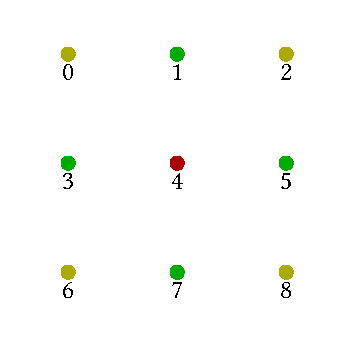
\includegraphics[width=0.33\textwidth]{./../appendix/lattice_visualization/square,size=2,np.pdf}}
            \makebox[0.40\textwidth][l]{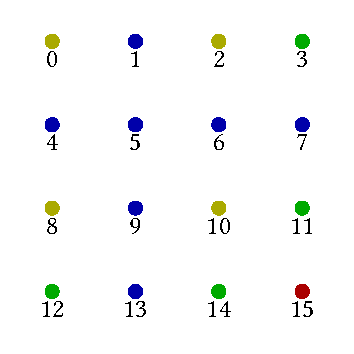
\includegraphics[width=0.33\textwidth]{./../appendix/lattice_visualization/square,size=3,p.pdf}}
            \makebox[0.40\textwidth][l]{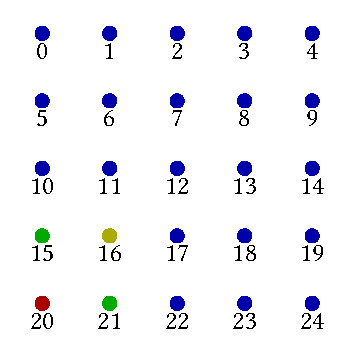
\includegraphics[width=0.33\textwidth]{./../appendix/lattice_visualization/square,size=4,np.pdf}}
        }
    }

    \captionof{figure}{A visualization of the \textbf{2D-square} lattice structure, measured in this thesis. 
        The lattices from left to right can be described by the parameters\\
        1: \emph{size=2, non-periodic}\,\,\,\, 2: \emph{size=3, periodic}\,\,\,\, 3: \emph{size=4, non-periodic}
    }
    \label{fig:appendix-square-lattices}
\end{minipage}

\vspace{0.5cm}

\begin{minipage}{\linewidth}
    \centering
    \makebox[\textwidth][c]{
        \makebox[1.25\textwidth][c]{
            \makebox[0.40\textwidth][l]{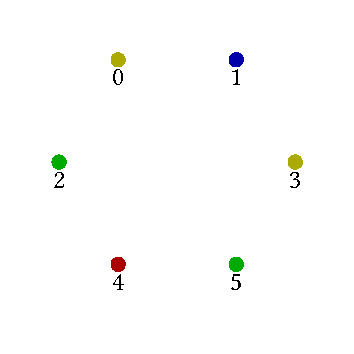
\includegraphics[width=0.33\textwidth]{./../appendix/lattice_visualization/hexagonal,size=1,np.pdf}}
            \makebox[0.40\textwidth][l]{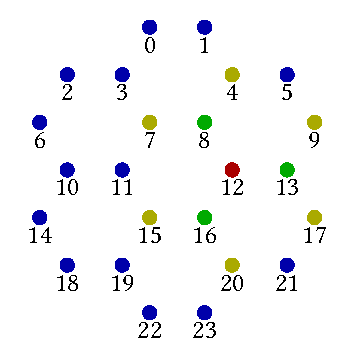
\includegraphics[width=0.33\textwidth]{./../appendix/lattice_visualization/hexagonal,size=2,np.pdf}}
            \makebox[0.40\textwidth][l]{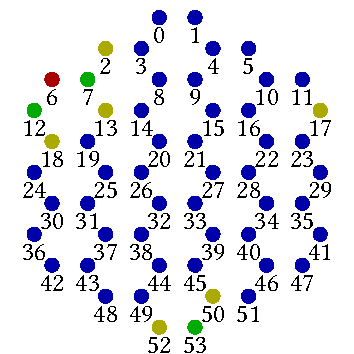
\includegraphics[width=0.33\textwidth]{./../appendix/lattice_visualization/hexagonal,size=3,p.pdf}}
        }
    }

    \vspace{0.3cm}
    \captionof{figure}{A visualization of the \textbf{2D-hexagonal} lattice structure, measured in this thesis. 
        The lattices from left to right can be described by the parameters \\
        1: \emph{size=1, non-periodic}\,\,\,\, 2: \emph{size=2, non-periodic}\,\,\,\, 3: \emph{size=3, periodic}
    }
    \label{fig:appendix-hexagonal-lattices}
\end{minipage}

\vspace{0.4cm}

\begin{minipage}{\linewidth}
    \centering
    \makebox[\textwidth][c]{
        \makebox[1.25\textwidth][c]{
            \makebox[0.40\textwidth][l]{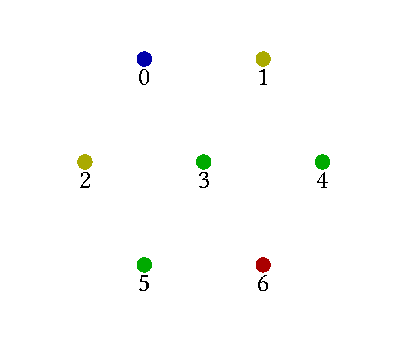
\includegraphics[width=0.33\textwidth]{./../appendix/lattice_visualization/trigonal_hexagonal,size=1,np.pdf}}
            \makebox[0.40\textwidth][l]{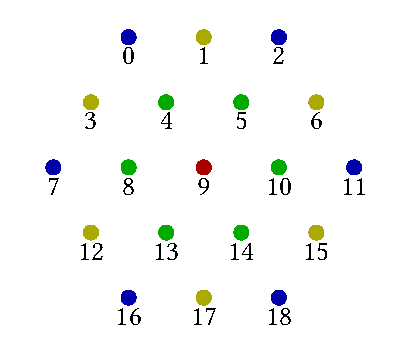
\includegraphics[width=0.33\textwidth]{./../appendix/lattice_visualization/trigonal_hexagonal,size=2,np.pdf}}
            \makebox[0.40\textwidth][l]{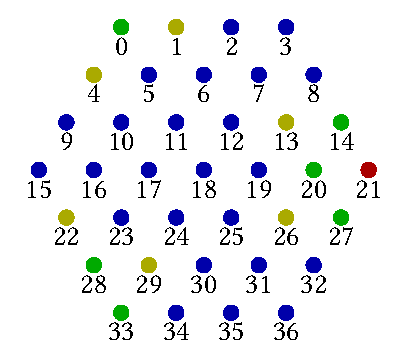
\includegraphics[width=0.33\textwidth]{./../appendix/lattice_visualization/trigonal_hexagonal,size=3,p.pdf}}
        }
    }
    
    \vspace{0.5cm}
    \captionof{figure}{A visualization of the \textbf{2D-trigonal\_hexagonal} lattice structure, measured in this thesis. 
        The lattices from left to right can be described by the parameters \\
        1: \emph{size=1, non-periodic}\,\,\,\, 2: \emph{size=2, non-periodic}\,\,\,\, 3: \emph{size=3, periodic}
    }
    \label{fig:appendix-trigonal_hexagonal-lattices}
\end{minipage}

% HERE SHOULD THE PAGE-BREAK BE. i love latex, but stuff like this infuriates me to get correct
\newpage
\makebox{\vspace{5cm}}\\

\begin{minipage}{\linewidth}
    \centering
    \makebox[\textwidth][c]{
        \makebox[1.25\textwidth][c]{
            \makebox[0.40\textwidth][l]{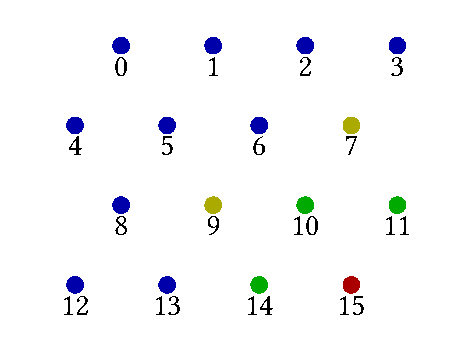
\includegraphics[width=0.33\textwidth]{./../appendix/lattice_visualization/trigonal_square,size=2,np.pdf}}
            \makebox[0.40\textwidth][l]{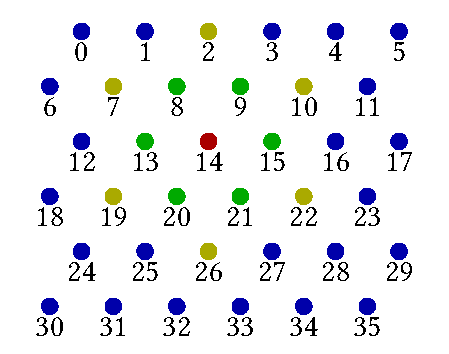
\includegraphics[width=0.33\textwidth]{./../appendix/lattice_visualization/trigonal_square,size=3,np.pdf}}
            \makebox[0.40\textwidth][l]{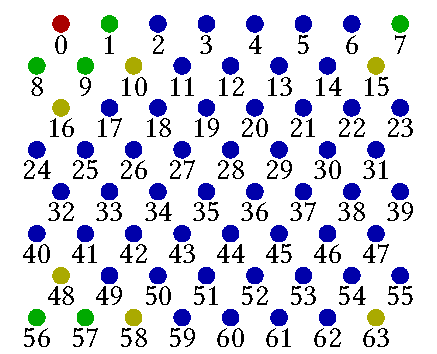
\includegraphics[width=0.33\textwidth]{./../appendix/lattice_visualization/trigonal_square,size=4,p.pdf}}
        }
    }

    \vspace{0.4cm}
    \captionof{figure}{A visualization of the \textbf{2D-trigonal\_square} lattice structure, measured in this thesis. 
        The lattices from left to right can be described by the parameters \\
        1: \emph{size=2, non-periodic}\,\,\,\, 2: \emph{size=3, non-periodic}\,\,\,\, 3: \emph{size=4, periodic}
    }
    \label{fig:appendix-trigonal_square-lattices}
\end{minipage}

\vspace{1.2cm}

\begin{minipage}{\linewidth}
    \centering
    \makebox[\textwidth][c]{
        \makebox[1.25\textwidth][c]{
            \makebox[0.40\textwidth][c]{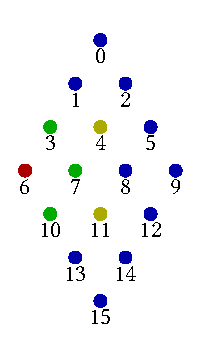
\includegraphics[width=0.20\textwidth]{./../appendix/lattice_visualization/trigonal_diamond,size=3,np.pdf}}
            \makebox[0.40\textwidth][c]{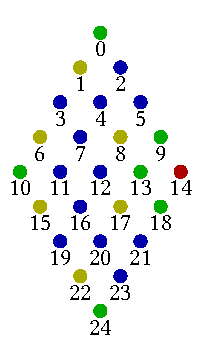
\includegraphics[width=0.20\textwidth]{./../appendix/lattice_visualization/trigonal_diamond,size=4,p.pdf}}
            \makebox[0.40\textwidth][c]{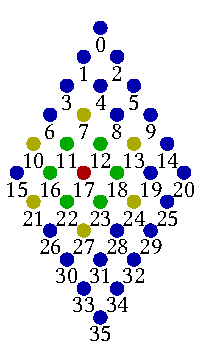
\includegraphics[width=0.20\textwidth]{./../appendix/lattice_visualization/trigonal_diamond,size=5,np.pdf}}
        }
    }

    \vspace{0.4cm}
    \captionof{figure}{A visualization of the \textbf{2D-trigonal\_diamond} lattice structure, measured in this thesis. 
        The lattices from left to right can be described by the parameters \\
        1: \emph{size=3, non-periodic}\,\,\,\, 2: \emph{size=4, periodic}\,\,\,\, 3: \emph{size=5, non-periodic}
    }
    \label{fig:appendix-trigonal_diamond-lattices}
\end{minipage}

\vspace{1.2cm}

\begin{minipage}{\linewidth}
    \centering
    \makebox[\textwidth][c]{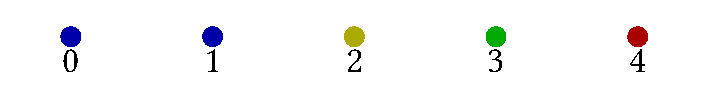
\includegraphics[width=0.80\textwidth]{./../appendix/lattice_visualization/linear,size=5,np.pdf}}
    \vspace*{0.2cm}
    \makebox[\textwidth][c]{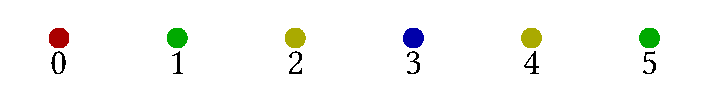
\includegraphics[width=0.80\textwidth]{./../appendix/lattice_visualization/linear,size=6,p.pdf}}
    \vspace*{0.2cm}
    \makebox[\textwidth][c]{
\includegraphics[width=0.80\textwidth]{./../appendix/lattice_visualization/linear,size=8,np.pdf}}

    \vspace{0.2cm}
    \captionof{figure}{A visualization of the \textbf{1D-linear} lattice structure, measured in this thesis. 
        The lattices from top to bottom can be described by the parameters \\
        1: \emph{size=5, non-periodic}\,\,\,\, 2: \emph{size=6, periodic}\,\,\,\, 3: \emph{size=8, non-periodic}
    }
    \label{fig:appendix-linear-lattices}
\end{minipage}

\newpage

% pdf as a additional information, can be nicely ref-ed ("\fullpage{anhang:test}") because of fake section that doesn't get shown in the table of contents
% \includepdf[pagecommand={\section*{} \label{appendix:test}}]{appendix/test.pdf}

% minted to properly import and style code. ! Needs python libraries
\newpage
\section{Dot Product Self Attention (jax)} \label{appendix:attention}
    \cite{selfPhysics}, \filepath{/models/metaformer.py}
    \inputminted[firstline=149, lastline=169]{python}{./../physics-code/models/metaformer.py}

\section{Graph Conformer Module (jax)} \label{appendix:graph-conformer}
    \cite{selfPhysics}, \filepath{/models/metaformer.py}
    \inputminted[firstline=242, lastline=284]{python}{./../physics-code/models/metaformer.py}

\newpage
\section{Graph Poolformer Module (jax)} \label{appendix:graph-poolformer}
    \cite{selfPhysics}, \filepath{/models/metaformer.py}
    \inputminted[firstline=211, lastline=239]{python}{./../physics-code/models/metaformer.py}
    

\end{document}





